\documentclass[11pt]{article}
\usepackage[margin=1in]{geometry}
\usepackage{graphicx,amsmath,amssymb,booktabs,siunitx,caption,subcaption}
\usepackage[hidelinks]{hyperref}
\usepackage{authblk}
\usepackage{xcolor}
\captionsetup{font=small,labelfont=bf}
\graphicspath{{fig/}}
\renewcommand{\arraystretch}{1.15}
\newcommand{\Csf}{C_{\mathrm{sf}}}
\newcommand{\Wcm}{\si{\watt\per\centi\meter\squared}}
\newcommand{\degC}{\si{\degreeCelsius}}

\title{\bfseries A Validated Reduced-Order Model for a Submerged Tube-Bundle Condenser
Pool-Boiling Chamber, with Manifold-Resolved Condenser CFD and its Link to Boiling-Curve Performance}
\author[1]{Thermal Analysis Laboratory}
\affil[1]{Department of Mechanical Engineering, Rochester Institute of Technology}
\date{\today}

\begin{document}
\maketitle

\begin{abstract}
\noindent
We report a validated gray-box reduced-order model for a closed subcooled pool-boiling
chamber cooled by a partially submerged tube-bundle condenser, a platform aimed at
two-phase immersion cooling of high-power electronics. Against \textbf{261 measured points}
spanning two condenser geometries (33- and 42-tube), two chip surfaces (plain and
microchannel), and four coolant inlet temperatures (\SIrange{20}{50}{\degreeCelsius}), the
model predicts chip temperature with an overall \textbf{$R^2=0.938$}, \textbf{RMSE
\SI{4.34}{\kelvin}}, and bias \SI{+0.89}{\kelvin}. The 33-tube plain configuration is
reproduced best ($R^2=0.964$, \SI{91}{\percent} of points within \SI{5}{\kelvin}), while the
42-tube configurations are weaker and biased high by \SI{\sim2}{\kelvin}. We then present
three-dimensional, STEP-faithful single-phase OpenFOAM simulations of the coolant manifolds
for all three condenser generations (33-, 42-, and 66-tube), which resolve the per-tube flow
distribution and the pressure budget. The simulations show that distribution and pressure
drop are governed by the \emph{manifold feed geometry and the tube bore size}, not the tube
count: a single centred port produces severe maldistribution while top-fed vertical manifolds
distribute evenly, and wide bores render the bundle hydraulically near-invisible while narrow
bores carry a measurable share of the drop. Finally we connect the two analyses: the
coolant-side thermal resistance that the manifold CFD informs is exactly the quantity that
sets the chamber saturation temperature and therefore the vertical position of the boiling
curve. This framework rationalises why the model is most robust for the wide-bore, high-flow
33-tube condenser (negligible coolant-side resistance) and weakest for the narrow-bore 42-tube
condenser (significant, distribution-sensitive coolant-side resistance).
\end{abstract}

\section{Introduction}
Direct two-phase immersion cooling is an attractive route to rejecting the rising heat fluxes
of data-center processors. The platform studied here is a closed chamber in which a heated chip
boils a subcooled dielectric pool; the vapour rises and condenses on a tube bundle that is
partially submerged in the same pool and carries a single-phase coolant. The chamber is
self-contained: the condenser sets the operating pressure (and hence the saturation
temperature) by balancing the vapour generated at the chip against the vapour condensed at the
bundle. Because the chip temperature at a given heat flux is the sum of the wall superheat and
the saturation temperature, condenser performance feeds directly into the achievable junction
temperature.

This paper has three goals. First, we summarise a reduced-order model of the chamber and
validate it against an extensive measurement set. Second, we use three-dimensional CFD to
resolve the coolant-side flow distribution in the condenser manifolds, which has not previously
been characterised for this apparatus. Third, and most importantly, we draw the physical link
between the manifold-resolved condenser behaviour and the measured boiling-curve performance,
giving a mechanistic explanation for where the reduced-order model is strong and where it is
weak.

\section{Apparatus and reduced-order model}
The model is a gray-box: established two-phase and single-phase correlations carry the physics,
and a small number of geometry-independent constants are fit once and then transferred across
configurations. Nucleate boiling on the chip is represented in the Rohsenow framework with a
surface--fluid constant $\Csf$; the microchannel surface is treated with area-enhancement and
the Cooke--Kandlikar description. The condenser side couples a tube-bundle condensation
resistance to a single-phase internal coolant resistance (Gnielinski/laminar developing flow
as appropriate) and an external bundle resistance. The chamber energy balance closes the loop:
for a heat load $Q$, the saturation temperature follows
\begin{equation}
T_{\mathrm{sat}} \;=\; T_{\mathrm{cool}} \;+\; Q\,R_{\mathrm{cond}},
\label{eq:tsat}
\end{equation}
where $R_{\mathrm{cond}}$ is the total condenser thermal resistance and $T_{\mathrm{cool}}$ the
coolant inlet temperature. The chip temperature is then
\begin{equation}
T_{\mathrm{surf}} \;=\; T_{\mathrm{sat}} \;+\; \Delta T_{\mathrm{sat}}(q),
\label{eq:tsurf}
\end{equation}
with the wall superheat $\Delta T_{\mathrm{sat}}$ set by the boiling correlation. A key design
property of this decomposition is that $\Csf$ is a property of the chip surface and the fluid,
not of the chamber: values fit on one condenser transfer to the other, which is what makes the
model predictive rather than a per-configuration curve fit.

\section{Experimental validation: model versus measurement}
Figure~\ref{fig:parity} compares predicted and measured chip temperature for all
\num{261} points. The predictions track the \num{1}:\num{1} line across the full
\SIrange{30}{120}{\degreeCelsius} range, with most points inside a \SI{\pm5}{\kelvin} band.
Table~\ref{tab:fit} reports the fit by configuration.

\begin{figure}[t]
\centering
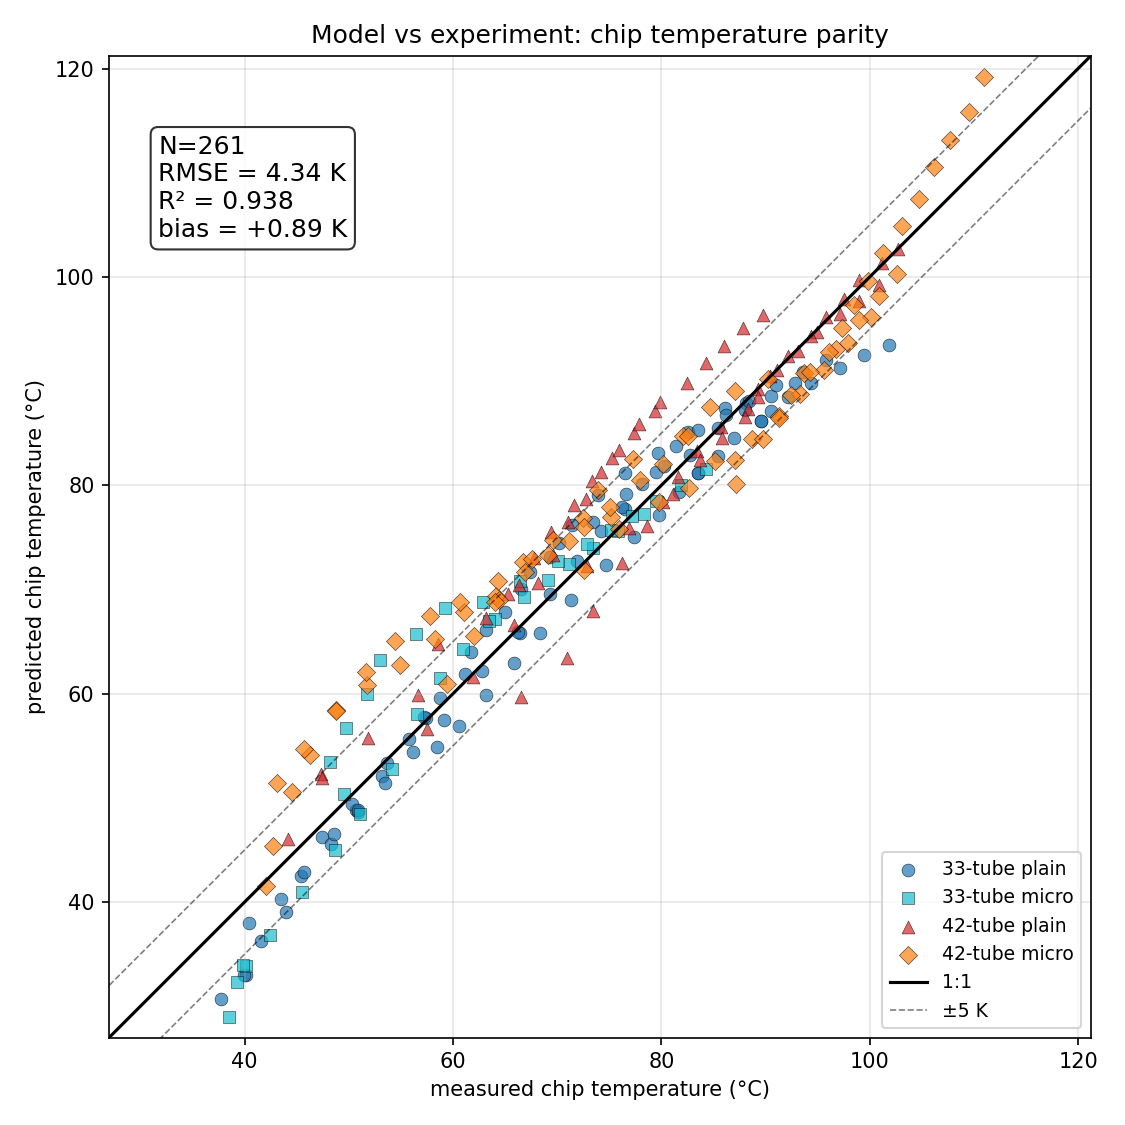
\includegraphics[width=0.62\linewidth]{me_parity.png}
\caption{Predicted versus measured chip temperature for all 261 points, by configuration.
The model achieves $R^2=0.938$ and RMSE \SI{4.34}{\kelvin}. The 33-tube data (blue/cyan) hug
the parity line; the 42-tube data (red/orange) sit slightly above it, reflecting a
\SI{+2}{\kelvin} bias.}
\label{fig:parity}
\end{figure}

\begin{table}[t]
\centering
\caption{Chip-temperature fit by configuration (in-sample). RMSE, MAE, bias and maximum
absolute residual in kelvin.}
\label{tab:fit}
\begin{tabular}{lrrrrrrr}
\toprule
Configuration & $N$ & RMSE & MAE & Bias & $R^2$ & $\max|r|$ & within \SI{5}{\kelvin}\\
\midrule
33-tube plain & 87 & 3.14 & 2.59 & $-0.99$ & 0.964 & 8.4 & \SI{91}{\percent}\\
33-tube micro & 36 & 4.82 & 3.85 & $+0.88$ & 0.867 & 10.2 & \SI{67}{\percent}\\
42-tube plain & 64 & 4.42 & 3.36 & $+2.00$ & 0.900 & 8.1 & \SI{66}{\percent}\\
42-tube micro & 74 & 5.17 & 4.47 & $+2.16$ & 0.927 & 10.6 & \SI{65}{\percent}\\
\midrule
\textbf{Overall} & \textbf{261} & \textbf{4.34} & \textbf{3.48} & \textbf{+0.89} & \textbf{0.938} & \textbf{10.6} & \textbf{74\%}\\
\bottomrule
\end{tabular}
\end{table}

The boiling-curve view (Figure~\ref{fig:boiling}) is more physically revealing than the parity
plot. For each configuration the measured heat flux is plotted against wall superheat
$T_{\mathrm{surf}}-T_{\mathrm{sat}}$ (filled markers), with the model prediction overlaid (open
markers), separated by coolant temperature. The model captures the entire coolant-temperature
\emph{family} of curves, including the rightward shift of the curve as the coolant warms. Two
features stand out and recur in the residuals (Figure~\ref{fig:resid}): the 33-tube panels
track tightly, whereas the 42-tube panels show systematic over-prediction of the superheat
(the open markers sit to the right of the filled markers).

\begin{figure}[t]
\centering
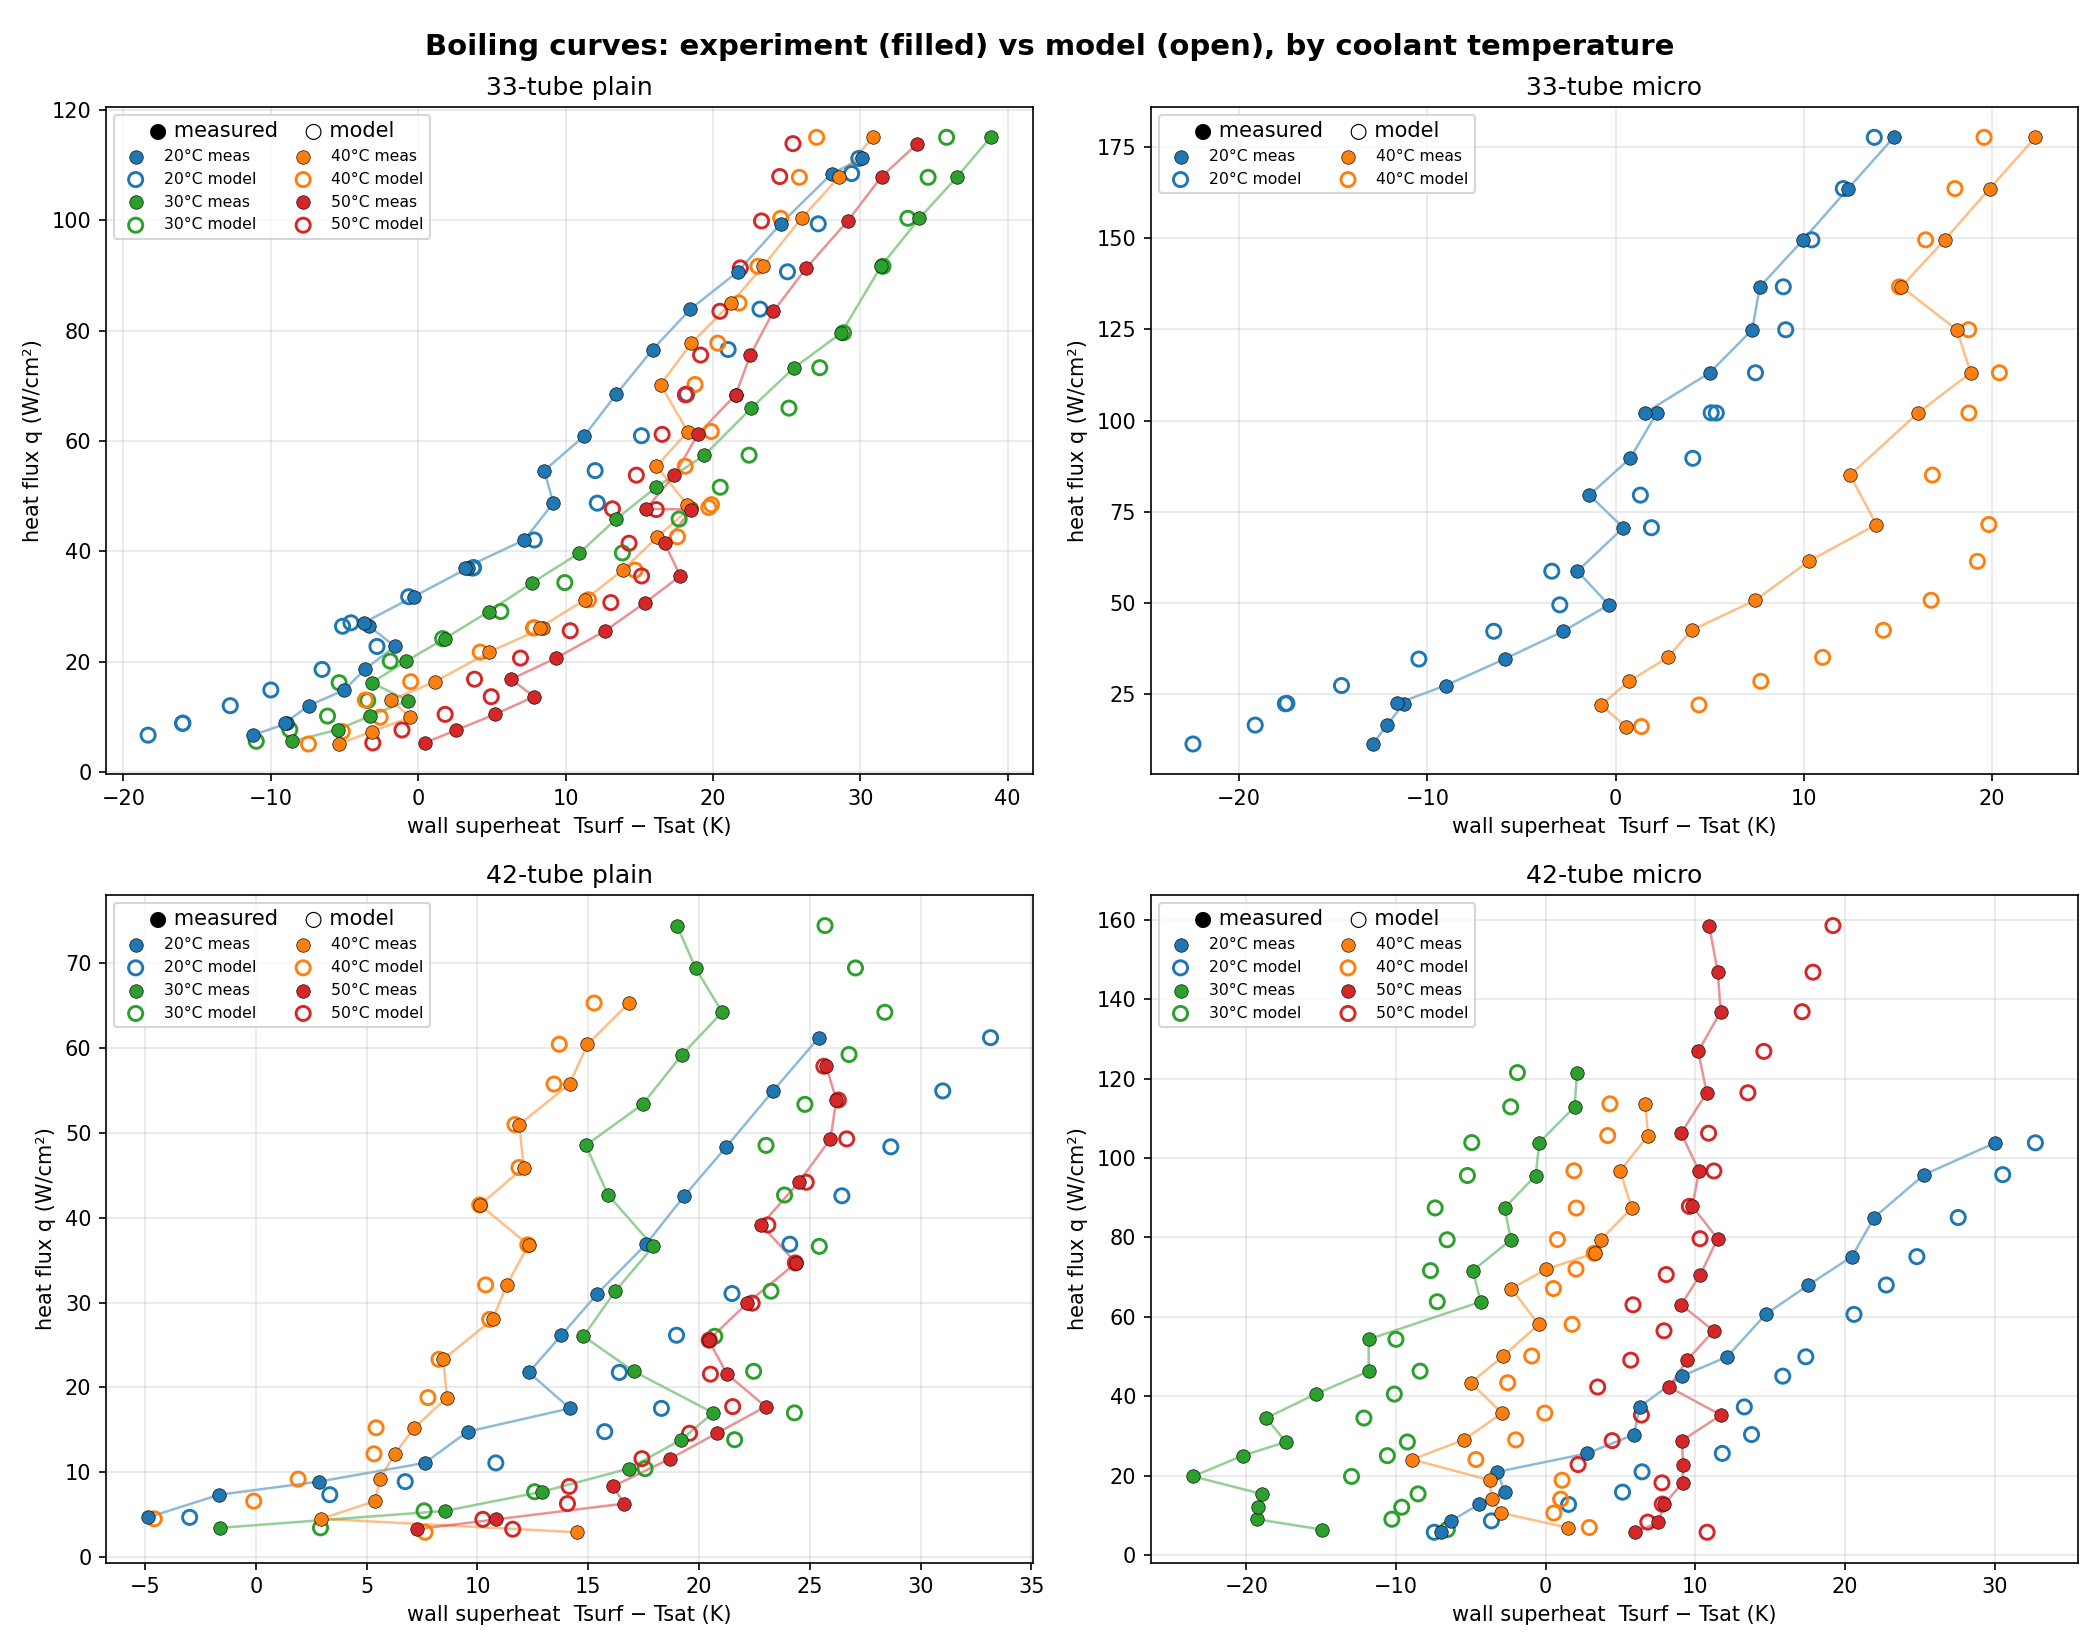
\includegraphics[width=\linewidth]{me_boiling.png}
\caption{Boiling curves, experiment (filled) versus model (open), by coolant temperature.
Heat flux versus wall superheat for each configuration. The model reproduces the
coolant-temperature family; agreement is tight for the 33-tube and looser, with a rightward
(over-prediction) offset, for the 42-tube.}
\label{fig:boiling}
\end{figure}

\begin{figure}[t]
\centering
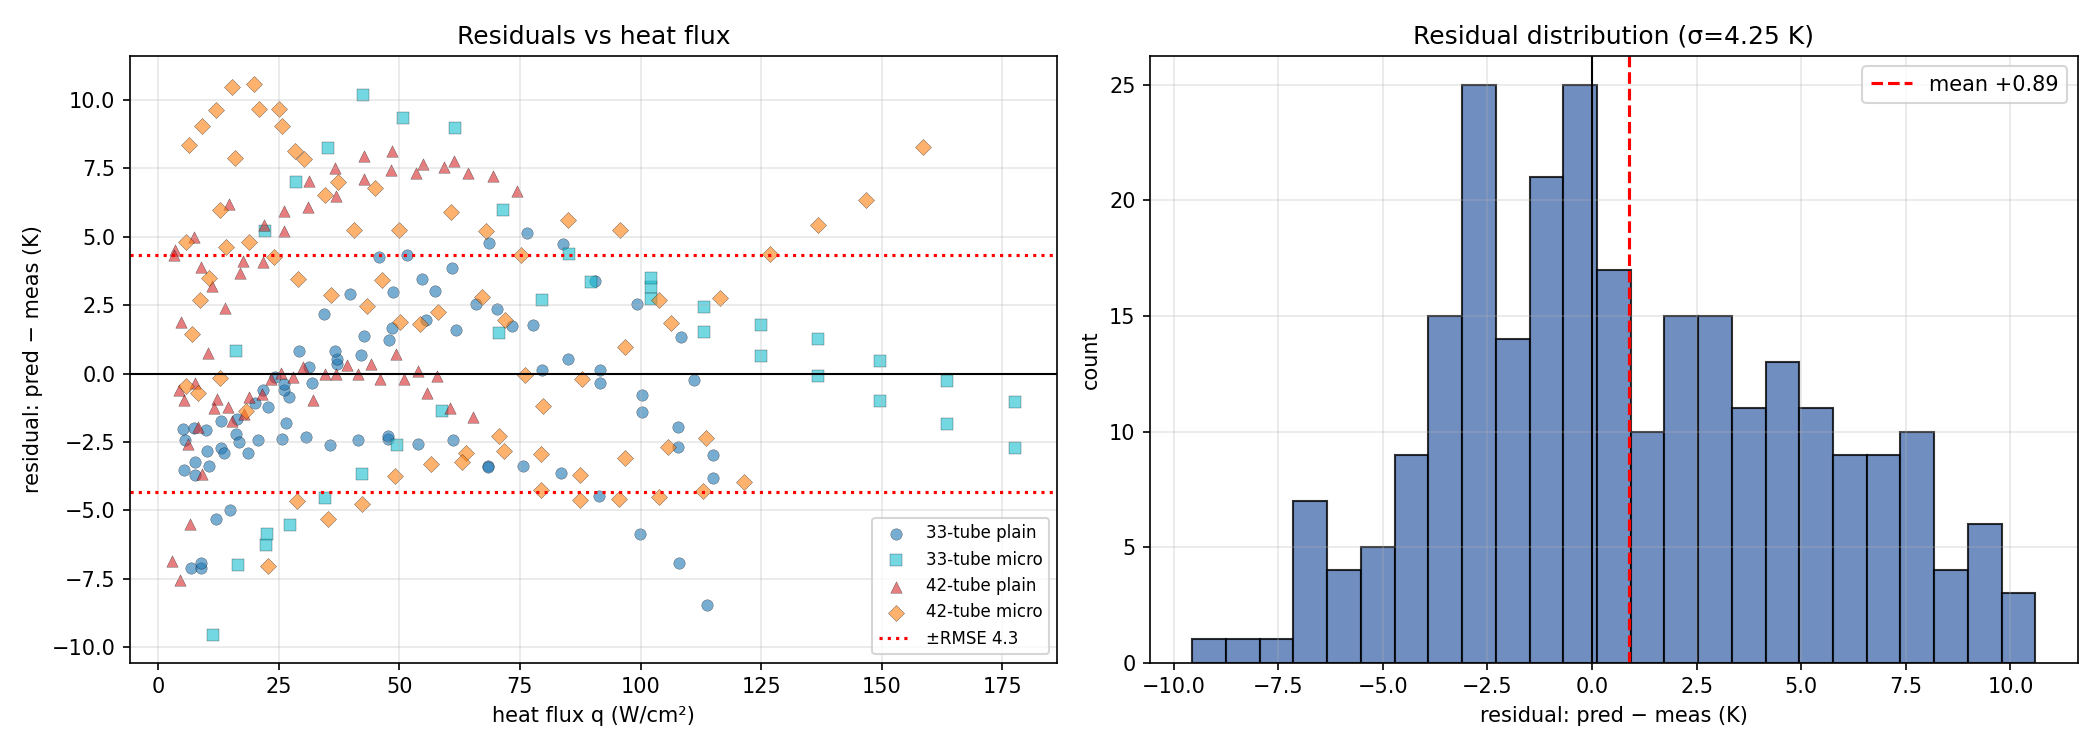
\includegraphics[width=\linewidth]{me_residuals.png}
\caption{Left: residuals versus heat flux, showing no systematic trend with flux, the model is
equally accurate at \SI{10}{} and \SI{170}{\Wcm}. Right: residual distribution
($\sigma=\SI{4.25}{\kelvin}$), centred near zero with a slight positive mean driven by the
42-tube.}
\label{fig:resid}
\end{figure}

Two diagnostics from the validation set are important for what follows. (i) The residuals show
\emph{no trend with heat flux}, which indicates the mechanistic correlations hold across the
boiling regime rather than being tuned at a single operating point. (ii) The bias is
\emph{coolant-temperature dependent}: warm coolant (\SIrange{40}{50}{\degreeCelsius}) is
reproduced best (RMSE \SI{\sim3.5}{\kelvin}) and the bias flips from \SI{+1.8}{\kelvin} at
\SI{20}{\degreeCelsius} to \SI{-1.4}{\kelvin} at \SI{50}{\degreeCelsius}. A sign change in the
bias with coolant temperature points to a residual in the \emph{coolant-side} description, a
clue that we return to in Section~\ref{sec:link}.

\section{Condenser manifold CFD}
The reduced-order condenser model lumps the coolant side into an effective resistance that
assumes the coolant is distributed across the tubes. Whether that assumption holds, and what
sets the pumping power, depends on the manifold hydraulics, which we resolve directly. For each
condenser generation we built a STEP-faithful single-phase fluid domain (manifold cavities plus
tube bores) from the production CAD and solved steady incompressible flow with \texttt{simpleFoam}
(laminar, water properties at \SI{\sim40}{\degreeCelsius}, \SI{4}{\litre\per\minute}). The three
geometries differ in tube count, bore size, and crucially in how the coolant is fed:

\begin{itemize}
\item \textbf{33-tube} (bore ID \SI{3.137}{\milli\meter}): a single coolant port on the bundle
axis, feeding the manifold centrally.
\item \textbf{42-tube} (bore ID \SI{1.39}{\milli\meter}): top-fed vertical manifolds at each
tube end, coolant entering and leaving through ports on the manifold tops.
\item \textbf{66-tube} (bore ID \SI{1.6}{\milli\meter}, forecast geometry): single-pass, fed
through a centreline port (modelled here with a simplified diffuser plenum).
\end{itemize}

\subsection{Per-tube distribution}
The distributions are strikingly different (Figure~\ref{fig:dist}). The 33-tube centred port
produces a \emph{bullseye}: a single on-axis tube is over-fed to roughly eight times the mean
while the rest are starved, giving a coefficient of variation $\mathrm{CoV}=\SI{131}{\percent}$.
The 42-tube top-fed manifolds, in contrast, distribute the coolant evenly,
$\mathrm{CoV}=\SI{10}{\percent}$, with only a mild bias toward the top-row tubes nearest the
inlet. The simplified 66-tube centreline feed shows an intermediate, jet-dominated pattern
($\mathrm{CoV}=\SI{57}{\percent}$) in which a few central tubes intercept the inlet jet; we
emphasise that this last figure is inflated by the simplified plenum and that the production
manifold is a lofted diffuser designed precisely to spread that jet (Section~\ref{sec:limits}).
All cases conserve mass to within the discretisation error.

\begin{figure}[t]
\centering
\begin{subfigure}{0.49\linewidth}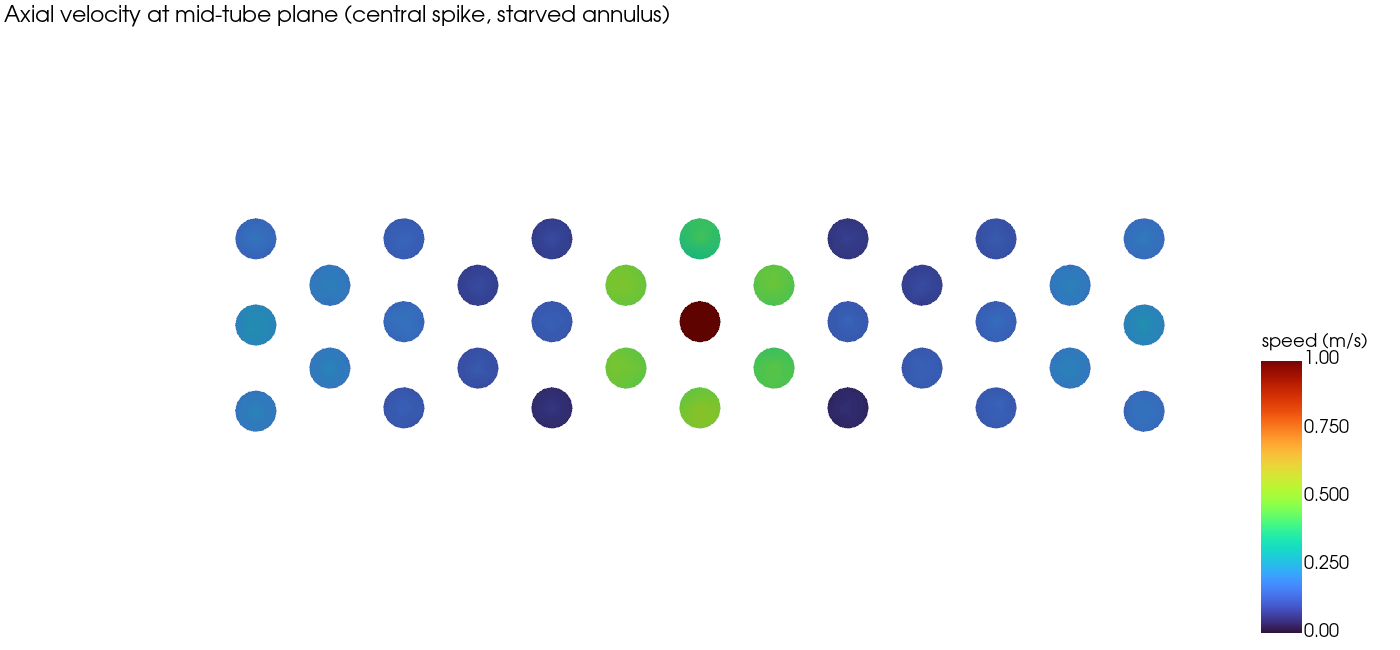
\includegraphics[width=\linewidth]{c33_cross.png}\caption{33-tube: bullseye, CoV \SI{131}{\percent}}\end{subfigure}\hfill
\begin{subfigure}{0.49\linewidth}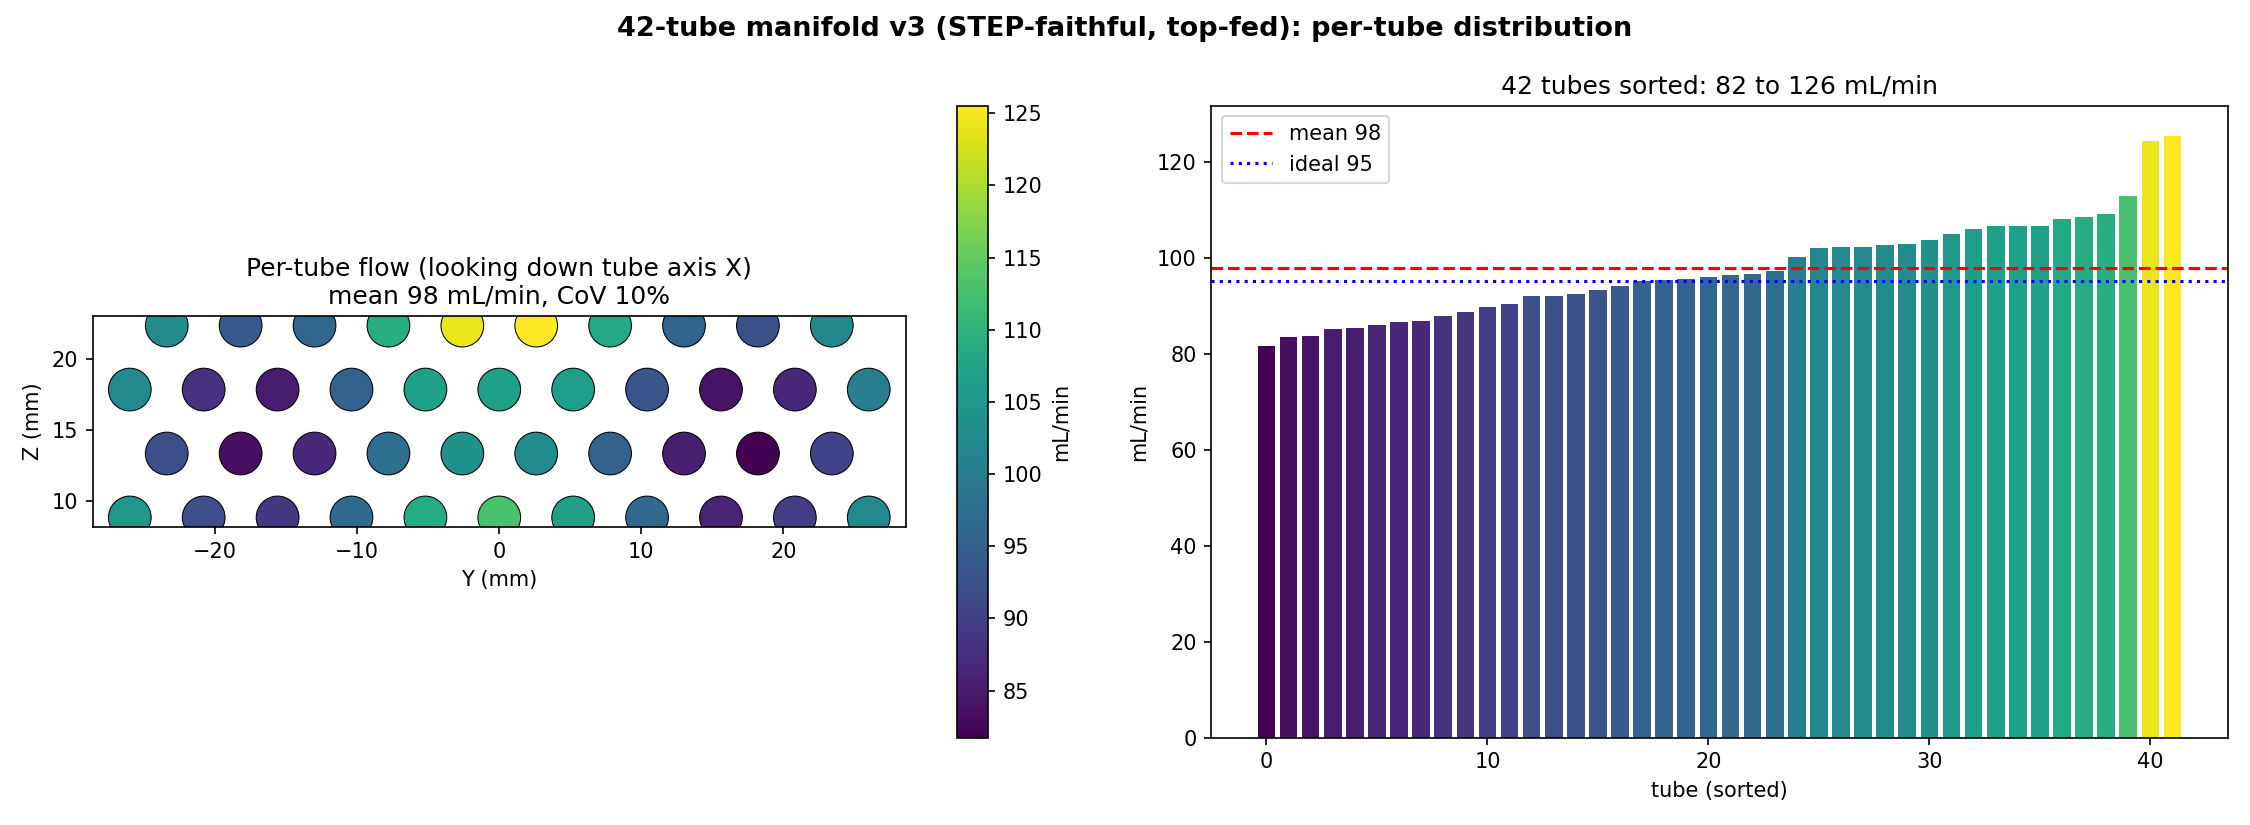
\includegraphics[width=\linewidth]{c42_dist.png}\caption{42-tube: uniform, CoV \SI{10}{\percent}}\end{subfigure}
\caption{Per-tube coolant distribution from CFD. A single centred port (33-tube, left) starves
all but the on-axis tube; top-fed vertical manifolds (42-tube, right) distribute evenly.
Distribution is governed by the manifold feed geometry, not the tube count.}
\label{fig:dist}
\end{figure}

\subsection{Pressure budget}
The pressure analysis (Figure~\ref{fig:press}) reveals a second bore-size effect. In the
wide-bore 33-tube condenser the pressure is essentially uniform through the entire bundle and
the full drop occurs across the small outlet port contraction: the tube bundle is
\emph{hydraulically near-invisible} (the tubes contribute \SI{\sim25}{\pascal} of a
\SI{\sim10}{\kilo\pascal} budget). In the narrow-bore 42-tube condenser the tubes carry a
\emph{measurable} share, \SI{\sim1.4}{\kilo\pascal} of distributed drop along the
\SI{62.6}{\milli\meter} length, although the port contractions still dominate. The 66-tube,
with wide bores split among many parallel paths, again behaves like the 33-tube with the drop
concentrated at the ports.

\begin{figure}[t]
\centering
\begin{subfigure}{0.49\linewidth}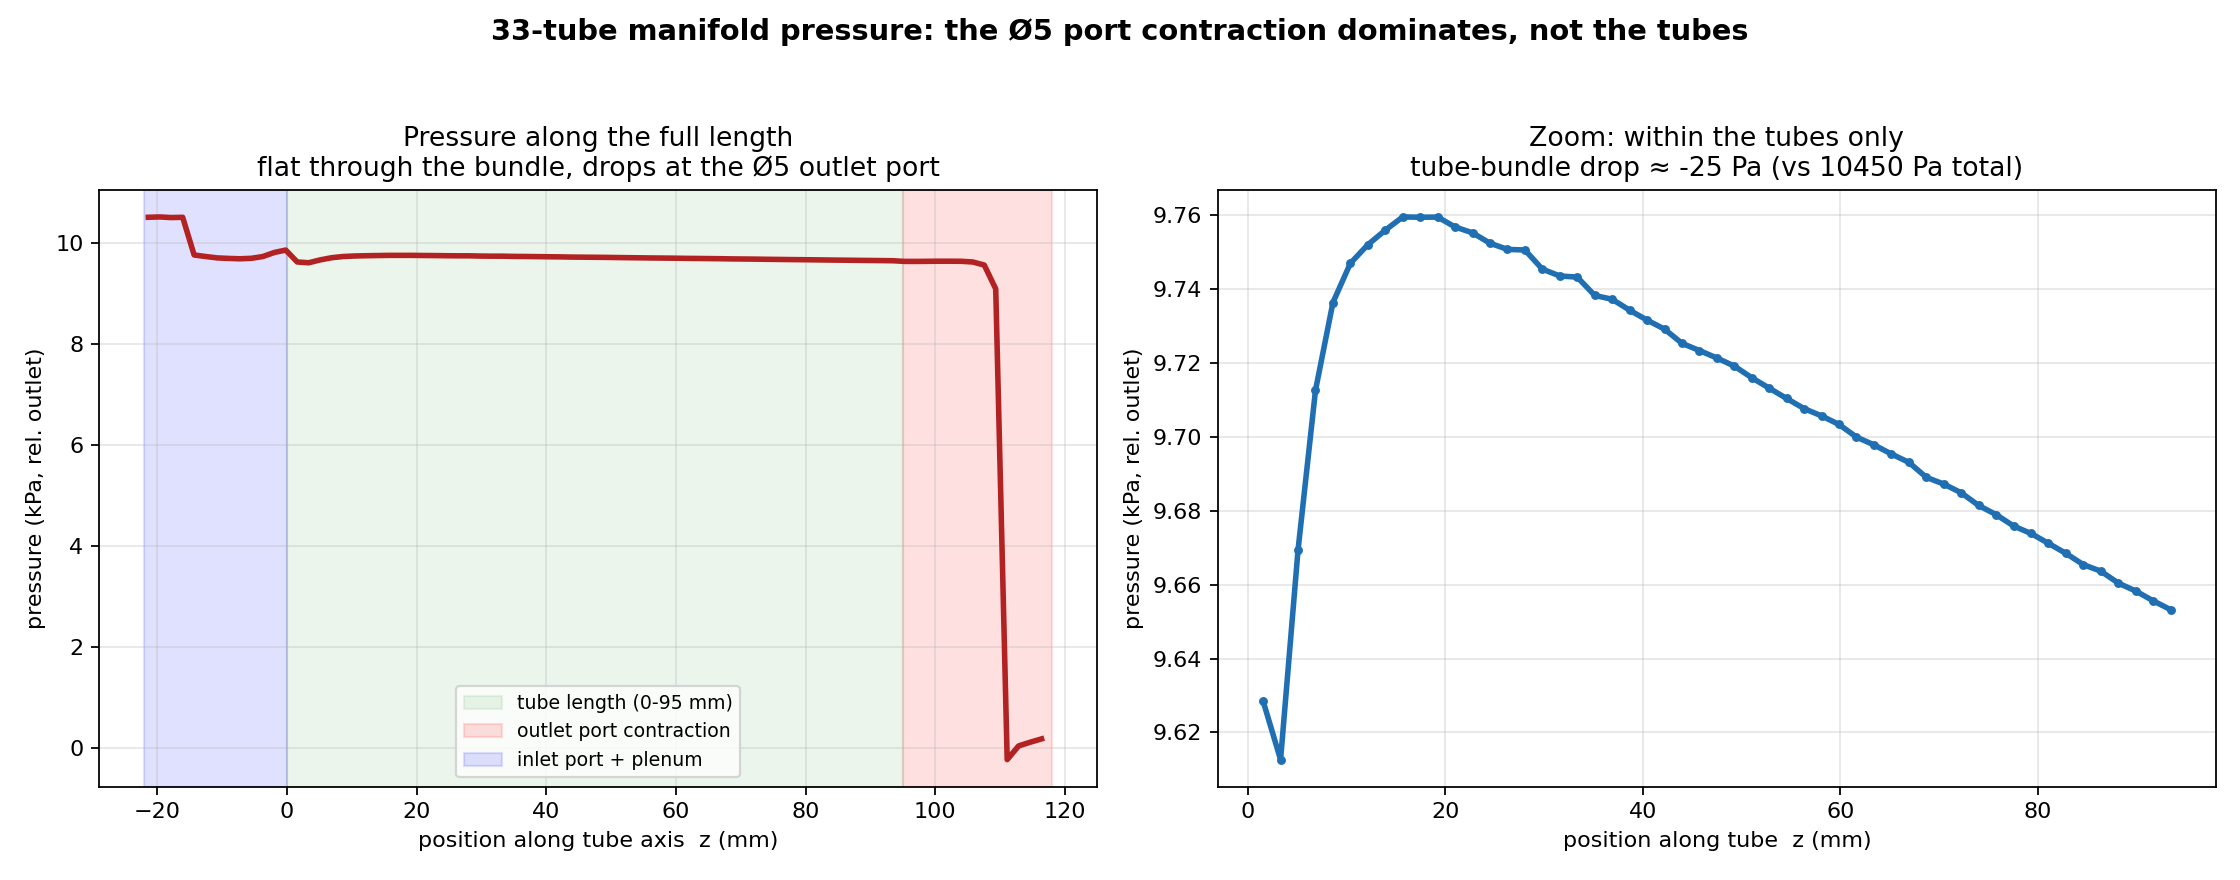
\includegraphics[width=\linewidth]{c33_press.png}\caption{33-tube: flat, drop at the port}\end{subfigure}\hfill
\begin{subfigure}{0.49\linewidth}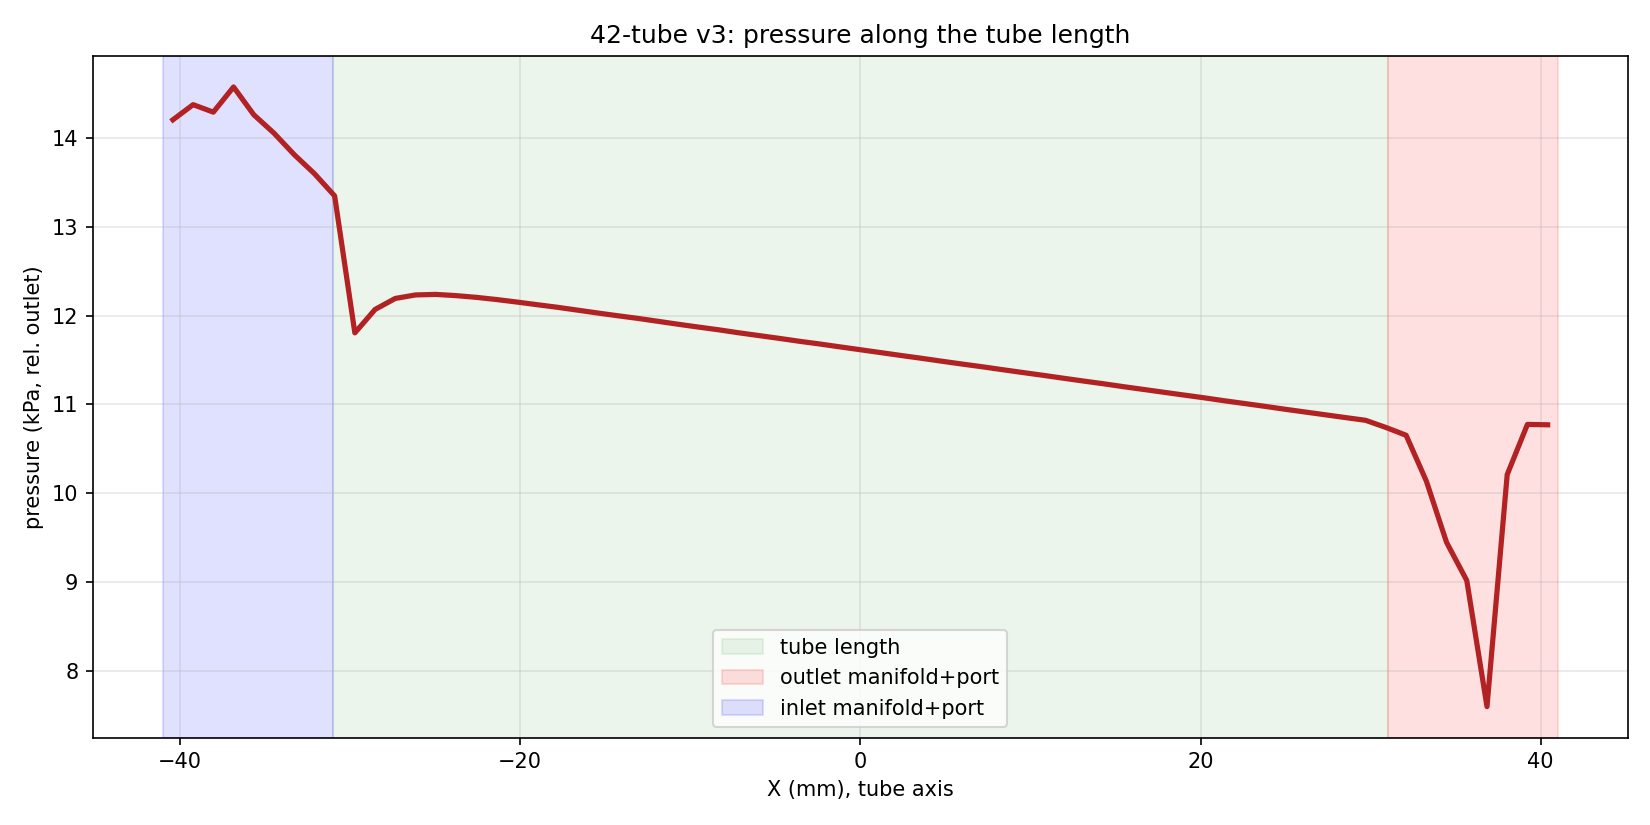
\includegraphics[width=\linewidth]{c42_press.png}\caption{42-tube: real drop along the tubes}\end{subfigure}
\caption{Pressure along the tube length. Wide bores (33-tube) leave the bundle hydraulically
near-invisible with the drop concentrated at the port contraction; narrow bores (42-tube) carry
a measurable distributed drop.}
\label{fig:press}
\end{figure}

\section{Linking condenser distribution to boiling-curve performance}
\label{sec:link}
The two analyses meet at the condenser thermal resistance $R_{\mathrm{cond}}$ in
Eq.~\eqref{eq:tsat}. The manifold CFD characterises the coolant side of that resistance; the
boiling-curve validation measures its consequence. The chain of causation is:
\begin{equation}
\underbrace{\text{manifold feed geometry}}_{\text{CFD}}
\;\rightarrow\; \text{per-tube coolant flow}
\;\rightarrow\; \underbrace{R_{\mathrm{cond}}}_{\text{Eq.~\eqref{eq:tsat}}}
\;\rightarrow\; T_{\mathrm{sat}}
\;\rightarrow\; \underbrace{T_{\mathrm{surf}}=T_{\mathrm{sat}}+\Delta T_{\mathrm{sat}}(q)}_{\text{boiling curve}} .
\label{eq:chain}
\end{equation}
A maldistributed manifold starves part of the bundle; starved tubes see their coolant warm
toward the local saturation temperature, lose driving $\Delta T$, and stop contributing
effective area. The effective conductance $UA$ falls, $R_{\mathrm{cond}}$ rises, and by
Eq.~\eqref{eq:tsat} the chamber runs at a higher $T_{\mathrm{sat}}$. Through
Eq.~\eqref{eq:tsurf} that lifts the entire boiling curve vertically: the chip runs hotter at
every heat flux. Manifold distribution is therefore not a hydraulic curiosity, it is a direct
lever on junction temperature.

The decisive subtlety is that the \emph{magnitude} of this lever depends on how large the
coolant-side resistance is relative to the rest of $R_{\mathrm{cond}}$, and this is exactly
what the bore-size pressure result foreshadows. The same property that makes the 33-tube bundle
hydraulically invisible, wide bores and a high coolant flow (\SI{0.06}{\kilo\gram\per\second}),
also makes its coolant-side \emph{thermal} resistance small: the coolant barely warms
($T_{\mathrm{out}}-T_{\mathrm{in}}$ is a fraction of a kelvin in the data), so even the severe
bullseye maldistribution moves $T_{\mathrm{sat}}$ very little. The condenser is over-capacity,
$R_{\mathrm{cond}}$ is dominated by terms insensitive to distribution, and the reduced-order
model is correspondingly robust, hence the best fit of any configuration ($R^2=0.964$).

The 42-tube condenser sits at the opposite extreme. Its narrow bores (ID
\SI{1.39}{\milli\meter}) and lower coolant flow make the internal coolant resistance a
significant fraction of $R_{\mathrm{cond}}$, the same physics that makes its tubes carry a real
pressure drop. The chamber saturation temperature is now genuinely sensitive to the per-tube
flow and to the developing-flow internal heat-transfer description, and small errors in the
coolant-side model translate directly into chip-temperature error. This offers a coherent,
mechanistic explanation for the otherwise puzzling pairing in
Table~\ref{tab:fit}: the configuration with the \emph{better} measured distribution (42-tube,
CoV \SI{10}{\percent}) is the \emph{harder} one to model, because its performance lives where
the coolant-side resistance matters. The coolant-temperature sign-flip in the 42-tube bias
(Section~3) is consistent with this reading: a residual in the internal-resistance or
subcooling treatment, amplified where the coolant side is not negligible.

This also clarifies how the manifold CFD should feed the reduced-order model. Where the
coolant-side resistance is negligible (wide-bore, high-flow), a lumped, uniformly distributed
$UA$ is adequate and the CFD simply confirms it. Where it is significant (narrow-bore), the
per-tube distribution from CFD can be folded into a distribution-weighted $UA$ rather than a
single bulk value, the most direct route to removing the 42-tube bias. For the forecast
66-tube, the lofted-diffuser manifold is expected to restore near-uniform distribution; the
simplified centreline-jet result should not be read as the apparatus prediction but as a
demonstration of why the diffuser is needed.

\section{Discussion and limitations}
\label{sec:limits}
The validation is in-sample on the two built condensers; leave-one-coolant-out
cross-validation (reported separately) shows stronger generalisation for the 33-tube than the
42-tube, consistent with the present fit. The manifold CFD is single-phase and steady, solved
on tetrahedral meshes to a mesh-limited residual plateau, and is intended to characterise
distribution and the pressure budget, not to be a converged high-fidelity solution. Two
geometric simplifications are explicit: the 42-tube manifold was modelled with its as-built
top ports, and the 66-tube inlet/outlet were simplified to a centreline-fed plenum rather than
the production lofted diffuser. The 66-tube geometry is a forecast with no validation data, so
all 66-tube results are exploratory. None of these simplifications affects the central
qualitative findings, that distribution is set by feed geometry, that bore size sets whether
the bundle carries hydraulic and thermal load, and that the coolant-side resistance is the
hinge linking condenser CFD to boiling-curve performance.

\section{Conclusions}
\begin{enumerate}
\item A gray-box reduced-order model reproduces chip temperature across two condensers, two
chip surfaces, and four coolant temperatures with $R^2=0.938$ and RMSE \SI{4.34}{\kelvin}; the
surface--fluid constant transfers across chambers, supporting a predictive rather than fitted
construction.
\item STEP-faithful manifold CFD shows that per-tube distribution is governed by the feed
geometry (a centred port gives CoV \SI{131}{\percent}; top-fed manifolds give CoV
\SI{10}{\percent}) and that bore size sets the pressure budget (wide bores leave the bundle
hydraulically near-invisible; narrow bores carry a real share).
\item The coolant-side thermal resistance links the two: it sets $T_{\mathrm{sat}}$ and hence
the vertical position of the boiling curve. The reduced-order model is most robust where this
resistance is negligible (wide-bore 33-tube) and weakest where it is significant
(narrow-bore 42-tube), giving a mechanistic explanation for the configuration-dependent fit and
a clear route to improvement: a distribution-weighted condenser conductance informed by the
manifold CFD.
\end{enumerate}

\paragraph{Data and reproducibility.} All model code is consolidated in a single
command-line tool; the CFD cases (geometry generators, meshes, run scripts, and solved fields)
and the figure-generating scripts are archived with the project.

\end{document}
